\documentclass[11pt]{article}
\usepackage[italian]{babel}
\usepackage{amsmath, amsfonts}
\usepackage{graphicx}
\begin{document}
\title{\Large Confronto tra gli algoritmi di ordinamento \textsc{Insertion-Sort} e \textsc{Quicksort}}\date{}
\author{Athos Innocenti}
\maketitle
\section{Introduzione}
Nella seguente relazione vengono presentati gli algoritmi di ordinamento \textsc{Insertion-Sort} e \textsc{Quicksort} e ne vengono comparate le prestazioni in funzione di vettori in input di dimensione crescente.

Per evidenziare al meglio l'andamento dei due algoritmi, i grafici si riferiscono a vettori di dimensione crescente fino a $4000$ incrementandola di $100$ ad ogni passo. Le tabelle, invece, fanno riferimento ad array di $10$, $100$, $1000$ elementi. Per ciascuna dimensione vengono eseguite $20$ prove.
\section{Insertion sort}
L'algoritmo di ordinamento \textsc{Insertion-Sort} ordina i numeri in input \textbf{sul posto}: i numeri sono risistemati all'interno dell'array \textit{A} senza richiedere ulteriore memoria aggiuntiva. Quando la procedura \textsc{Insertion-Sort}  è completata, l'array \textit{A} contiene la sequenza ordinata.

I tempi di esecuzione di \textsc{Insertion-Sort} nei tre casi sono:
\begin{description}
\item[Caso peggiore]Si verifica quando gli elementi del vettore in input sono ordinati al contrario.\\Il tempo di esecuzione di \textsc{Insertion-Sort} è $T(n) = \Theta(n^2)$
\item[Caso medio]Il tempo di esecuzione è $T(n) = \Theta(n^2)$
\item[Caso migliore]Si verifica quando gli elementi nel vettore sono già correttamente ordinati.\\Il tempo di esecuzione è dato da $T(n) = \Theta(n)$
\end{description}
\subsection{Analisi del caso peggiore}
Come si può notare dai tempi riportati in tabella \ref{t_peggiore_insertion} e dal grafico in figura \ref{peggiore_insertion}, nel caso peggiore di \textsc{Insertion-Sort} il tempo di esecuzione dell'algoritmo cresce in modo quadratico rispetto alla dimensione dell'array.
\begin{table}[h]
\centering
\begin{tabular}{|c|c|c|c|}\hline
Dimensione &10 &100 &1000\\ \hline
Prova 1	&1.001e-05 &1.788e-05 &1.648e-04 \\ \hline
Prova 2	&3.099e-06	&1.597e-05 &1.741e-04 \\ \hline
Prova 3	&2.146e-06	&1.596e-05 &1.699e-04 \\ \hline
Prova 4	&2.145e-06	&1.598e-05 &1.801e-04	 \\ \hline
Prova 5	&3.099e-06	&1.602e-05 &1.759e-04 \\ \hline
Prova 6	&2.861e-06 &1.621e-05 &1.691e-04  \\ \hline
Prova 7	&1.907e-06	&1.502e-05 &1.711e-04 \\ \hline
Prova 8	&1.908e-06	&1.478e-05 &1.762e-04	 \\ \hline
Prova 9	&2.146e-06	&1.692e-05 &1.658e-04 \\ \hline
Prova 10&1.907e-06 &1.597e-05 &1.903e-04 \\ \hline
\end{tabular}
\caption{Tempi di esecuzione nel caso peggiore di \textsc{Insertion-Sort}}
\label{t_peggiore_insertion}
\end{table}
\begin{figure}[h]
\centering
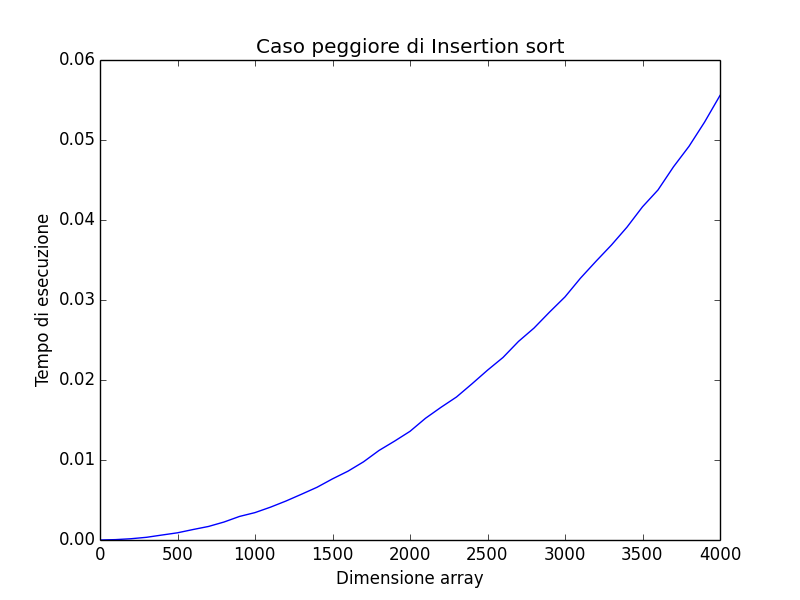
\includegraphics[scale=0.33,angle=0]{peggiore_insertion.png}
\caption{Caso peggiore di \textsc{Insertion-Sort}}
\label{peggiore_insertion}
\end{figure}
\subsection{Analisi del caso medio}
Nel caso medio di \textsc{Insertion-Sort}, come si vede nella tabella \ref{t_medio_insertion} e in figura \ref{medio_insertion}, il tempo di esecuzione è asintoticamente uguale al tempo di esecuzione nel caso peggiore; ovvero una crescita quadratica in relazione alla dimensione dell'array in input da ordinare.
\begin{table}[h]
\centering
\begin{tabular}{|c|c|c|c|}\hline
Dimensione &10 &100 &1000\\ \hline
Prova 1	&5.961e-06	&2.942e-04 &3.358e-02 \\ \hline
Prova 2	&5.007e-06	&3.271e-04	&3.322e-02 \\ \hline
Prova 3	&5.006e-06 &3.011e-04	&3.351e-02 \\ \hline
Prova 4	&4.053e-06	&3.309e-04	&3.327e-02	 \\ \hline
Prova 5	&5.961e-06	&3.559e-04	&3.266e-02 \\ \hline
Prova 6	&6.199e-06	&3.111e-04	&3.411e-02  \\ \hline
Prova 7	&5.007e-06	&3.491e-04	&3.241e-02  \\ \hline
Prova 8	&6.914e-06	&2.871e-04	&3.308e-02	 \\ \hline
Prova 9	&4.768e-06	&3.273e-04	&3.204e-02	 \\ \hline
Prova 10&5.007e-06 &3.758e-04	&3.322e-02	\\ \hline
\end{tabular}
\caption{Tempi di esecuzione nel caso medio di \textsc{Insertion-Sort}}
\label{t_medio_insertion}
\end{table}
\begin{figure}[h]
\centering
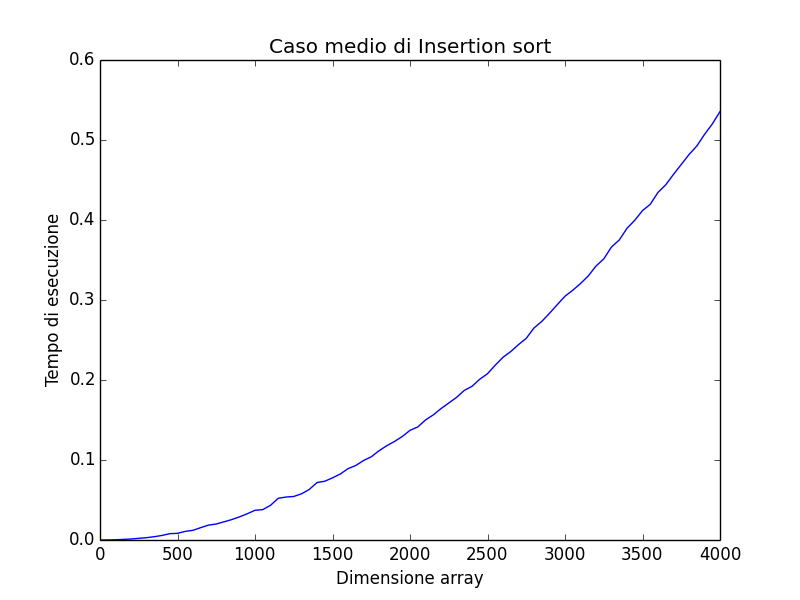
\includegraphics[scale=0.33,angle=0]{medio_insertion.png}
\caption{Caso medio di \textsc{Insertion-Sort}}
\label{medio_insertion}
\end{figure}\\
\subsection{Analisi del caso migliore}
Il caso migliore di \textsc{Insertion-Sort} si verifica quando i valori sono già ordinati nel modo corretto. In tal caso, come si può vedere dai tempi di esecuzione riportati nella tabella \ref{t_migliore_insertion} e dalla figura \ref{migliore_insertion}, il tempo di esecuzione dell'algoritmo cresce linearmente rispetto alla dimensione dell'array in input da ordinare.
\begin{table}[h]
\centering
\begin{tabular}{|c|c|c|c|}\hline
Dimensione &10 &100 &1000\\ \hline
Prova 1	&4.053e-06	&1.597e-05 &1.571e-04 \\ \hline
Prova 2	&2.146e-06	&1.598e-05	&1.619e-04 \\ \hline
Prova 3	&3.099e-06	&1.502e-05	&1.631e-04 \\ \hline
Prova 4	&1.907e-06	&1.716e-05	&1.621e-04 \\ \hline
Prova 5	&1.907e-06	&1.502e-05	&1.631e-04 \\ \hline
Prova 6	&1.908e-06	&1.503e-05	&1.649e-04  \\ \hline
Prova 7	&2.146e-06	&1.621e-05	&1.648e-04  \\ \hline
Prova 8	&1.907e-06	&1.597e-05	&1.649e-04 \\ \hline
Prova 9	&1.907e-06	&1.599e-05	&1.628e-04 \\ \hline
Prova 10&3.099e-06	&1.596e-05 &1.618e-04 \\ \hline
\end{tabular}
\caption{Tempi di esecuzione nel caso migliore di \textsc{Insertion-Sort}}
\label{t_migliore_insertion}
\end{table}
\begin{figure}[h]
\centering
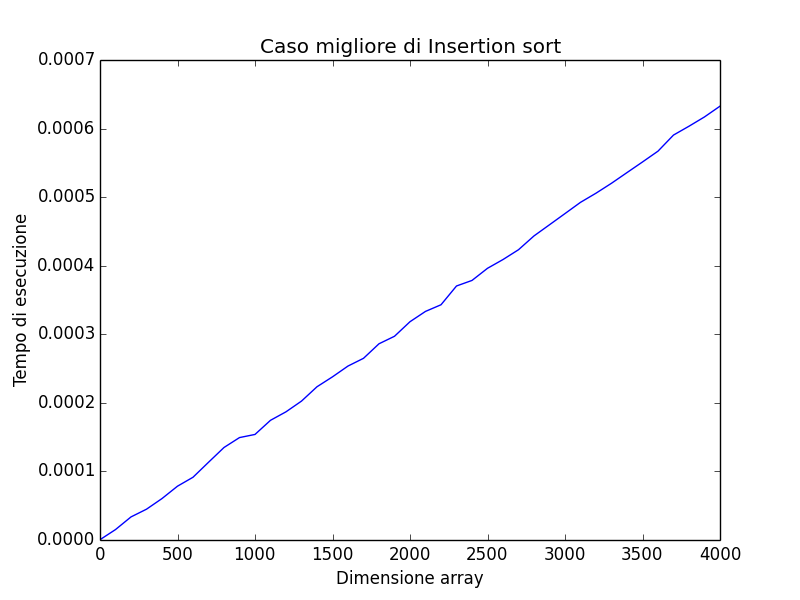
\includegraphics[scale=0.33,angle=0]{migliore_insertion.png}
\caption{Caso migliore di \textsc{Insertion-Sort}}
\label{migliore_insertion}
\end{figure}
\section{Quicksort}
\textsc{Quicksort} è un algoritmo di ordinamento ricorsivo basato sul paradigma \textit{divide et impera}. I tempi di esecuzione di \textsc{Quicksort} nei tre casi sono:
\begin{description}
\item[Caso peggiore]Si verifica quando \textsc{Partition} produce un sottoproblema con \textit{n - 1} elementi e uno con 0 elementi.\\Il tempo di esecuzione di \textsc{Quicksort} è $T(n) = \Theta(n^2)$
\item[Caso medio]Il tempo di esecuzione è $T(n) = \Theta(n\,lg\,n)$
\item[Caso migliore]Si verifica nel caso di bilanciamento massimo ovvero quando \textsc{Partition} produce due sottoproblemi, ciascun di dimensione non maggiore di $n/2$ (uno ha dimensione $\lfloor n/2 \rfloor$, l'altro $\lceil n/2 \rceil - 1$).\\Il tempo di esecuzione di \textsc{Quicksort} è $T(n) = \Theta(n\,lg\,n)$
\end{description}
\subsection{Analisi del caso medio}
Il tempo di esecuzione del caso medio di \textsc{Quicksort}, che lo si può pensare come l'alternanza di taglio buoni (ripartizione bilanciata - caso migliore) e tagli cattivi (ripartizione completamente sbilanciata - caso peggiore), è come il tempo di esecuzione nel caso in cui le ripartizioni generate da \textsc{Partition} sono soltanto buone: $O(n\,lg\,n)$ ma con una costante un po' più grande nascosta nella notazione \textit{O}. Tale andamento lo si può riscontrare nei tempi riportati in tabella \ref{t_medio_quick} e in figura \ref{medio_quick}.
\begin{table}[h]
\centering
\begin{tabular}{|c|c|c|c|}\hline
Dimensione &10 &100 &1000\\ \hline
Prova 1	&1.287e-05	&1.531e-04 &1.891e-03 \\ \hline
Prova 2	&1.844e-06	&1.321e-04	&1.816e-03 \\ \hline
Prova 3	&1.821e-06	&1.222e-04	&1.891e-03 \\ \hline
Prova 4	&1.002e-05	&1.371e-04	&1.878e-03	 \\ \hline
Prova 5	&1.003e-05	&1.432e-04 &1.969e-03 \\ \hline
Prova 6	&1.786e-06	&1.471e-04&1.873e-03  \\ \hline
Prova 7	&1.811e-06	&1.528e-04	&1.847e-03  \\ \hline
Prova 8	&1.001e-05	&1.419e-04	&1.817e-03 \\ \hline
Prova 9	&1.002e-05	&1.431e-04	&1.804e-03	 \\ \hline
Prova 10&1.867e-06	&1.501e-04 &1.834e-03\\ \hline
\end{tabular}
\caption{Tempi di esecuzione nel caso medio di \textsc{Quickort}}
\label{t_medio_quick}
\end{table}
\begin{figure}[h]
\centering
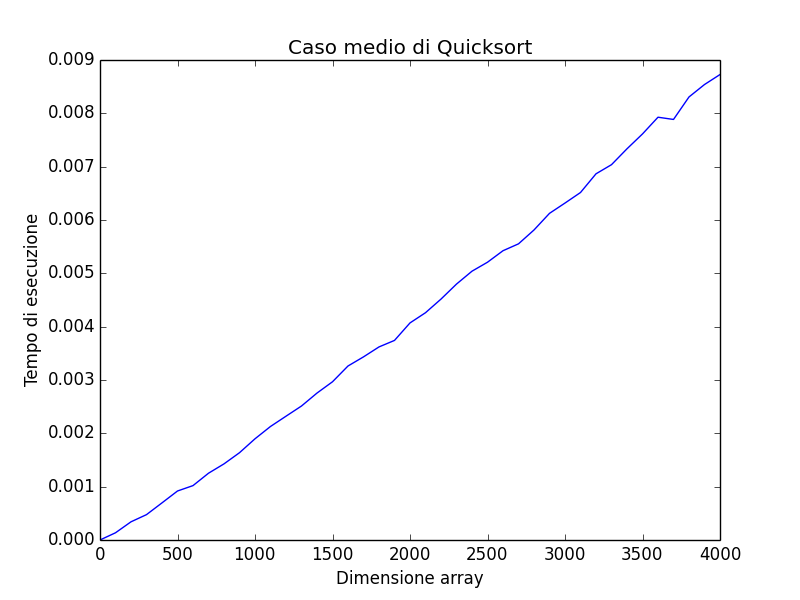
\includegraphics[scale=0.33,angle=0]{medio_quicksort.png}
\caption{Caso medio di \textsc{Quicksort}}
\label{medio_quick}
\end{figure}
\section{Confronto tra Insertion sort e Quicksort}
\subsection{Confronto nel caso medio}
Come si può osservare in figura \ref{medio_confronto}, nel caso di un array in input da ordinare composto da numeri casuali, rappresentante il caso medio dei due algoritmi, l'algoritmo \textsc{Quicksort} è molto più veloce di \textsc{Insertion-Sort}.
\begin{figure}[h]
\centering
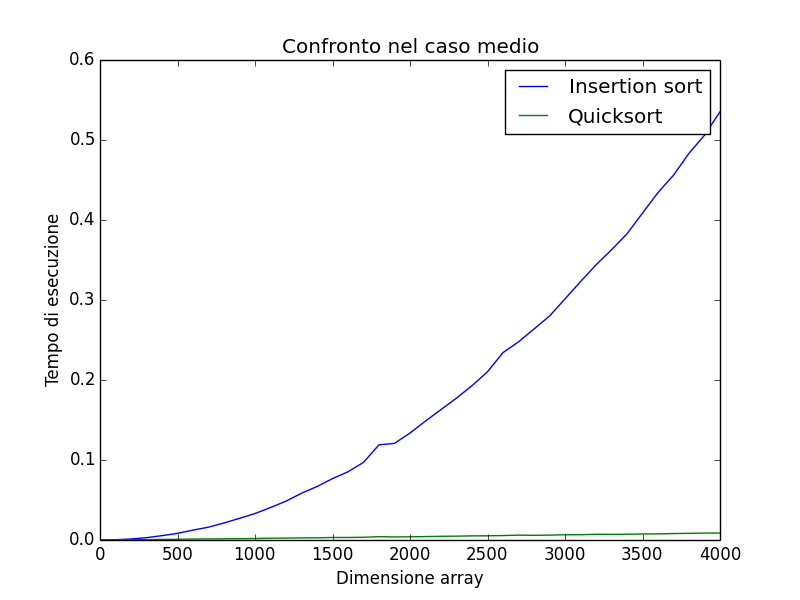
\includegraphics[scale=0.33,angle=0]{medio_confronto.png}
\caption{Confronto nel caso medio}
\label{medio_confronto}
\end{figure}
\subsection{Quicksort nel caso migliore e peggiore di Insertion sort}
Il caso migliore e peggiore di \textsc{Insertion-Sort} corrispondono, rispettivamente, al caso di un array già ordinato e un array ordinato al contrario. Entrambi i casi rientrano nel caso peggiore di \textsc{Quicksort} in quanto la procedura \textsc{Partition} produrrà uno sbilanciamento massimo con un sottoarray completamente vuoto e l'altro contenente tutti i valori.

Come si può verificare dai grafici in figura \ref{migliore_confronto} e \ref{peggiore_confronto}, il tempo di esecuzione di \textsc{Quicksort} nel caso di array già ordinato o ordinato al contrario cresce come $O(n^2)$ in funzione della dimensione \textit{n} del vettore in input da ordinare risultando essere più lento di \textsc{Insertion-Sort}.

\textsc{Insertion-Sort} nel caso peggiore di \textsc{Quicksort} corrisponde al caso migliore o peggiore di \textsc{Insertion-Sort} già stato analizzato.
\newpage
\begin{figure}[h]
\centering
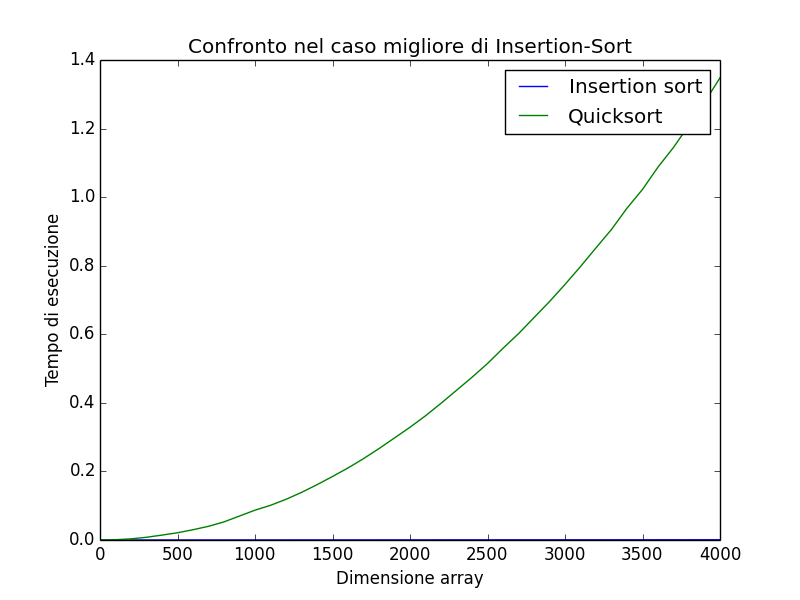
\includegraphics[scale=0.33,angle=0]{migliore_confronto.png}
\caption{Confronto nel caso migliore di \textsc{Insertion-Sort}}
\label{migliore_confronto}
\centering
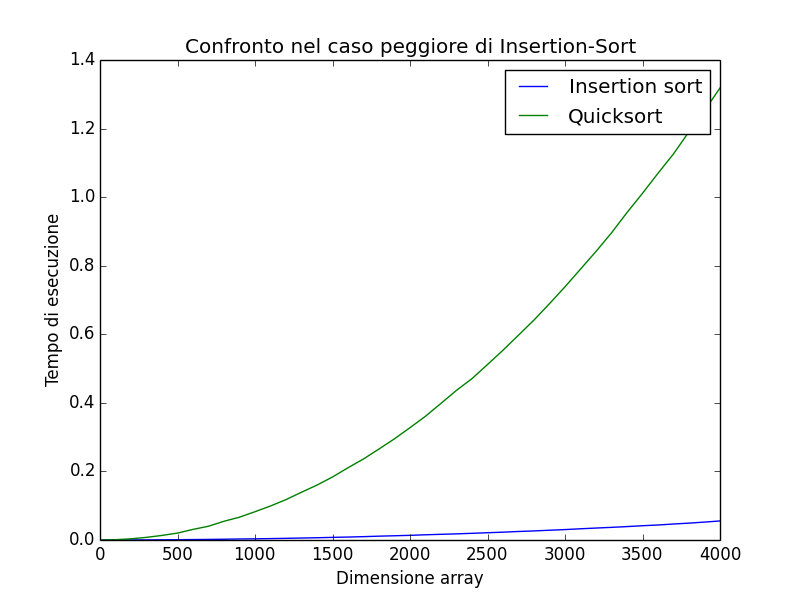
\includegraphics[scale=0.33,angle=0]{peggiore_confronto.png}
\caption{Confronto nel caso peggiore di \textsc{Insertion-Sort}}
\label{peggiore_confronto}
\end{figure}
\section{Conclusioni}
Tramite i vari test è stato possibile verificare i risultati teorici attesi. Come è stato possibile verificare dai vari esperimenti, la dimensione dell'array in input da ordinare nonché l'ordinamento iniziale dei valori influenzano il tempo di esecuzione dei due algoritmi. Si è dimostrato che \textsc{Quicksort} è più veloce in quasi tutti i casi in esame, poiché il suo caso medio è molto più vicino al caso migliore piuttosto che al peggiore, al contrario di \textsc{Insertion-Sort}.

I test sono stati eseguiti su un Macbook Pro con processore 2,7 GHz Intel Core i5, RAM 8 GB 1867 MHz DDR3 e sistema operativo macOS Mojave 10.14.6.
\end{document}